\documentclass[a4paper]{article}

% Packages
% ========

\usepackage{emposter}
\usepackage{multicol}

% EM-poster template settings
% ===========================

% title in the poster heading (auto centered)
\title{%
Example poster for the Graduate School Engineering Mechanics%
}
% author in the poster heading (auto centered)
\author{%
T.W.J.\ de Geus$^2$, J.\ van Beeck$^2$, \\
R.A.M.F.\ van Outvorst$^1$, J.A.W.\ van Dommelen$^{1,2}$%
}
% corresponding affiliations in the poster heading
\affiliation{%
$^1$Graduate School Engineering Mechanics\\%
$^2$Eindhoven University of Technology%
}

% university logo, in footer (left)
\university{
\includegraphics[height=1.0\logoheight]{tue}}
% additional logo's, in footer (right)
\rightlogo{
\includegraphics[height=1.0\logoheight]{stw}\hspace{5mm}
\includegraphics[height=1.0\logoheight]{stw}}

% progress bar in the footer (center):
% title (e.g. MSc, PhD, or PostDoc)
\progresstype{MSc/PhD/Postdoc~progress}
% total number of progress sections (years)
\progresssections{4}
% fraction of the bar to be filled
\progressfraction{32/48}

% %%%%%%%%%%%%%%%%%%%%%%%%%%%%%%%%%%%%%%%%%%%%%%%%
\begin{document}
\maketitle
% %%%%%%%%%%%%%%%%%%%%%%%%%%%%%%%%%%%%%%%%%%%%%%%%
\begin{multicols}{2}

% ================================================
\section{Introduction}
% ================================================

An example of the EM graduate school poster style is shown

% ================================================
\section{Logos}
% ================================================

The logos of the primary affiliation (i.e.\ the university) and the other affiliations and sponsors of the project are included at the bottom of the poster, respectively at the left and the right. They are included by
\begin{verbatim}
  \university{...}
  \rightlogo{...}
\end{verbatim}
whereby in principle any \LaTeX-code can be used at the dots. A common usage is
\begin{verbatim}
  \university{%
    \includegraphics[height=\logoheight]{...}%
  }
  \rightlogo{%
    \includegraphics[height=\logoheight]{...}%
  }
\end{verbatim}

% ================================================
\section{Preamble}
% ================================================

The title, authors, and their affiliations are included in the poster by the
\begin{verbatim}
  \title{...}
  \author{...}
  \affiliation{...}
\end{verbatim}
commands in the preamble of the document.

The progress bar in the footer is included using:
\begin{verbatim}
  \progresstype{...}
  \progresssections{...}
  \progressfraction{...}
\end{verbatim}
which creates a progress bar in the footer. The command respectively set the title, number of fields, and the fraction of the bar to fill.

The rest of the \LaTeX-code has the following structure:
\begin{verbatim}
  \begin{document}
  \maketitle
  ...
  \end{document}
\end{verbatim}

% ================================================
\section{Column layout}
% ================================================

The poster can be divided in multiple columns. For example the following code can is used to create the two columns of this example
\begin{verbatim}
  \begin{document}
  \maketitle
  \begin{multicols}{2}
  ...
  \end{multicols}
  \end{document}
\end{verbatim}
Alternative, one could also use mini-pages:
\begin{verbatim}
  \begin{document}
  \maketitle
  \begin{minipage}[t]{0.48\textwidth}
  ...
  \end{minipage}
  \hfill
  \begin{minipage}[t]{0.48\textwidth}
  ...
  \end{minipage}
  \end{document}
\end{verbatim}
or other constructions.

% ================================================
\section{Body}
% ================================================

The regular \LaTeX-commands can be used, e.g.\
\begin{verbatim}
  \section{...}
\end{verbatim}

Similarly figures can can be included as follows
\begin{verbatim}
  \begin{figure}[H]
    \includegraphics[height=6mm]{...}
    \caption{...}
  \end{figure}
\end{verbatim}

% ================================================
\section{Example}
% ================================================

Example text generated by \cite{lipsum}

Lorem ipsum dolor sit amet, consectetur adipiscing elit. Phasellus nec lectus quis ipsum adipiscing rhoncus non quis orci. Pellentesque a molestie velit. Pellentesque vel nisl nibh. Suspendisse at metus id nibh ultricies dapibus. Nunc nec eros ut justo malesuada ultricies a sed lectus. Phasellus id neque commodo est iaculis elementum nec nec magna. Vestibulum commodo, nibh vel adipiscing bibendum, sem quam congue velit, vitae porta risus augue et nibh. Vestibulum ante ipsum primis in faucibus orci luctus et ultrices posuere cubilia Curae.

% ------------------------------------------------
\begin{figure}[H]
\centering
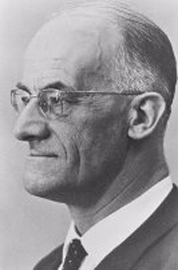
\includegraphics[height=4cm]{Koiter.jpg}
\caption{Warner Tjardus Koiter.}
\end{figure}
% ------------------------------------------------

% ================================================
% references
% ================================================

\begin{thebibliography}{99}
\bibitem{lipsum}
  http://www.lipsum.com/feed/html
\end{thebibliography}

\end{multicols}
% %%%%%%%%%%%%%%%%%%%%%%%%%%%%%%%%%%%%%%%%%%%%%%%%
\end{document}
% %%%%%%%%%%%%%%%%%%%%%%%%%%%%%%%%%%%%%%%%%%%%%%%%